\documentclass[]{article}
\usepackage[a4paper]{geometry}
\usepackage[dutch]{babel}

% Floating figuren.
\usepackage{graphicx}

% Commented, want we gebruiken dit eigenlijk niet?
%\usepackage{titling}

% Om code en dergelijke te plaatsen.
\usepackage{listings}

% Wiskundige formules in LaTeX <3
\usepackage{amsmath}
\usepackage{amssymb}
\usepackage{amsfonts}

% MATRICES! :D
\usepackage{amsmath}
\setcounter{MaxMatrixCols}{25} 

% Ik vind het nu eenmaal mooier zo.
\setlength{\parindent}{0pt}
\setlength{\parskip}{14pt}

\title{Project Datacommunicatie}
\author{Enver Bral \\
        Fr\'ed\'erique De Baerdemaeker \\
        Ruben Taelman \\
        Felix Van der Jeugt}
\date{Academiejaar 2012 - 2013}

\begin{document}
\maketitle

\begin{section}*{Broncodering}

    \begin{subsection}*{Vraag 1}

        We verkrijgen volgende output bij het uitvoeren van
        \texttt{FrequencyCounter.m}:

        \begin{lstlisting}
            0.5443    0.0024    0.0031    0.0040
            0.0019    0.0045    0.0001    0.0026
            0.0020    0.0001    0.0044    0.0029
            0.0045    0.0025    0.0018    0.4189
        \end{lstlisting}

        Dit zijn de relatieve frequenties voor elk macroblok. De
        macroblokken zijn hier als volgt genummerd: We zetten de rijen
        van het macroblok na elkaar, en lezen als een binair getal.  Zo
        wordt het macroblock \texttt{[1 0;0 1]} omgezet naar
        \texttt{1 0 0 1} en krijgt het nummer $9$.

        Met deze frequenties kunnen we de huffman-boom opstellen. Deze
        vindt u in Figuur~\ref{fig:manual_huffman}. Door aan de
        vertakking met het kleinste deelgewicht een nul toe te kennen,
        en een \'e\'en anders, bekomen we de codering in
        Tabel~\ref{tab:manual_huffman}.

        \begin{figure}
            \centering
            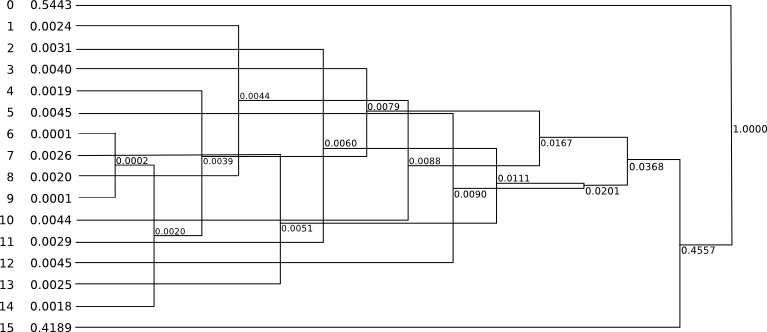
\includegraphics[width=\textwidth]{manual_huffman.png}
            \caption{Huffmanboom, opgesteld bij de frequenties uit
            \label{fig:manual_huffman}
            vraag 1.}
        \end{figure}

        \begin{table}
            \centering
            \begin{tabular}{lr@{.}lr}
                \textbf{Macrosymbool} & \multicolumn{2}{l}{\textbf{Rel. freq.}} &
                \textbf{Codewoord} \\
                \hline
                \texttt{0000} & 54 & 43 \% & \texttt{1} \\
                \texttt{0001} &  0 & 24 \% & \texttt{000101} \\
                \texttt{0010} &  0 & 31 \% & \texttt{001111} \\
                \texttt{0011} &  0 & 40 \% & \texttt{00001} \\
                \texttt{0100} &  0 & 19 \% & \texttt{000000} \\
                \texttt{0101} &  0 & 45 \% & \texttt{00100} \\
                \texttt{0110} &  0 & 01 \% & \texttt{00000100} \\
                \texttt{0111} &  0 & 26 \% & \texttt{001101} \\
                \texttt{1000} &  0 & 20 \% & \texttt{000100} \\
                \texttt{1001} &  0 & 01 \% & \texttt{00000101} \\
                \texttt{1010} &  0 & 44 \% & \texttt{00011} \\
                \texttt{1011} &  0 & 29 \% & \texttt{001110} \\
                \texttt{1100} &  0 & 45 \% & \texttt{00101} \\
                \texttt{1101} &  0 & 25 \% & \texttt{001100} \\
                \texttt{1110} &  0 & 18 \% & \texttt{0000011} \\
                \texttt{1111} & 41 & 89 \% & \texttt{01} \\
            \end{tabular}
            \caption{De Huffmancode bij vraag 1.}
            \label{tab:manual_huffman}
        \end{table}

        Nu kunnen we het gemiddeld aantal codebits per bronsymbool
        eenvoudig berekenen:

        \begin{eqnarray*}
            \mathbb{E}(n)
            &=& \frac{1}{4} \sum^{16}_{i=1}{p_i c_i} \\
            &=& \frac{1}{4*100}(1*54.43 + 6*0.24 + 6*0.31 + 5*0.40
                + 6*0.19 + 5*0.45 + 8*0.01 \\ && + 6*0.26 + 6*0.20
                + 8*0.01 + 5*0.44 + 6*0.29 + 5*0.45 + 6*0.25 \\ &&
                + 7*0.18 + 2*41.89) \\
            &=& \frac{158.77}{400} \\
            &=& 0.396925
        \end{eqnarray*}

        De afbeelding kan dus tot amper 40 procent van zijn
        oorspronkelijke grootte gereduceerd worden met behulp van
        Huffman codering.

    \end{subsection}

    \begin{subsection}*{Vraag 3}

        We verkrijgen volgende grafiek bij het uitvoeren van
        \texttt{vraag1\_3.m}:

        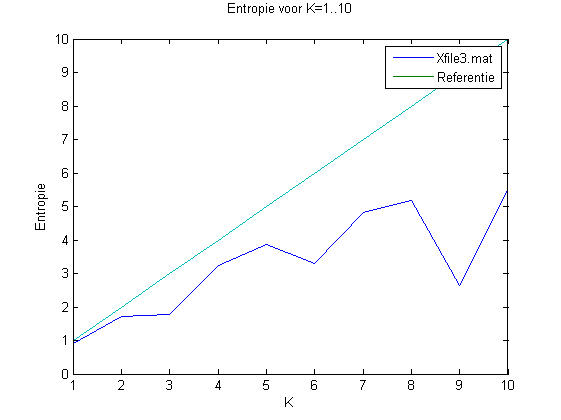
\includegraphics{vraag1_3.png}

        Hierop kunnen we de entropie zien van de macrosymbolen van
        grootte K. De referentielijn is hier een rechte, dit is logisch
        aangezien de entropie maximaal is wanneer alle symbolen met
        gelijke kans voorkomen.
        Vanaf K=8 komen er symbolen voor die met frequentie 0
        voorkomen, dus hier is de log2 -oneindig, dus de entropie wordt
        hier ook oneindig groot.

    \end{subsection}

    \begin{subsection}*{Vraag 4}

        We verkrijgen volgende grafiek bij het uitvoeren van
        \texttt{vraag1\_4.main()}:

        \begin{figure}[h]
            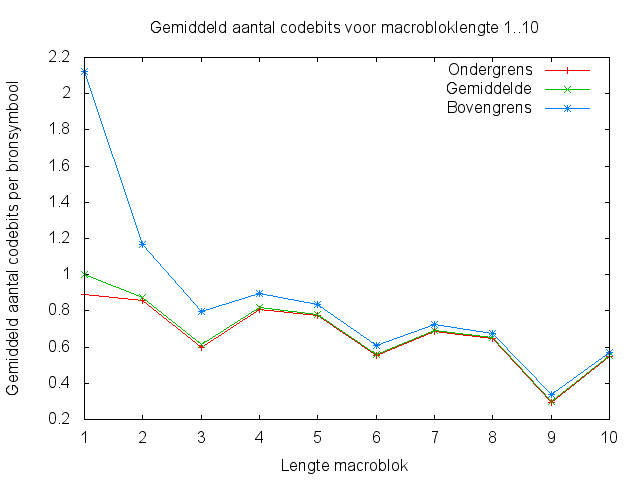
\includegraphics[scale=0.75]{vraag1_4.png}
            \caption{Het gemiddeld aantal codebits per bronsymbool in
            functie van de lengte van een macroblok.}
            \label{fig:codebits}
        \end{figure}

        Hierop kunnen we het gemiddelde aantal codebits per bronsymbool
        (gebruikmakend van huffmancodering) voor macrosymbolen met
        grootte K=1..10 en de bijhorende onder/bovengrens.

        % We nemen best 3 bits samen om het bestand optimaal te
        % comprimeren, we zouden ook eventueel 6 kunnen nemen met als
        % gevolg dat het coderen aanzienlijk trager verloopt.
        % We krijgen een compressiefactor van TBA
		
    \end{subsection}

    \begin{subsection}*{Vraag 5}

        In Figuur~\ref{fig:codebits} zien we dat $\mathbb{E}[n]$ zeer
        dicht bij de ondergrens ligt. Enkel voor macroblokken van
        grootte \'e\'en is dit niet het geval, maar aangezien we geen
        codewoorden van korter dan \'e\'en bit kunnen toekennen, is dit
        slechts te verwachten. Dit kleine verschil wijst erop dat
        Huffmancodering een zeer goede broncodering is.

        % TODO: Optimaal? Voorwaarden?

    \end{subsection}
    
    \begin{subsection}*{Vraag 6}
    	
    	Vertrekkende van de \emph{niet-canonische} Huffman codes in 
    	tabel~\ref{tab:manual_huffman}, vinden we de canonische
    	Huffman codes gegeven in tabel~\ref{tab:canonical_huffman}
    	
    	\begin{table}
            \centering
            \begin{tabular}{c|r}
                \textbf{Macrosymbool} &
                \textbf{Codewoord} \\
                \hline
                \texttt{0000} & \texttt{0} \\
				\texttt{0001} & \texttt{111000} \\
				\texttt{0010} & \texttt{111001} \\
				\texttt{0011} & \texttt{11000} \\
				\texttt{0100} & \texttt{111010} \\
				\texttt{0101} & \texttt{11001} \\
				\texttt{0110} & \texttt{11111110} \\
				\texttt{0111} & \texttt{111011} \\
				\texttt{1000} & \texttt{111100} \\
				\texttt{1001} & \texttt{11111111} \\
				\texttt{1010} & \texttt{11010} \\
				\texttt{1011} & \texttt{111101} \\
				\texttt{1100} & \texttt{11011} \\
				\texttt{1101} & \texttt{111110} \\
				\texttt{1110} & \texttt{1111110} \\
				\texttt{1111} & \texttt{10} \\
            \end{tabular}
            \caption{Canonische Huffmancodes bij vraag 6}
            \label{tab:canonical_huffman}
        \end{table}
    	
    \end{subsection}

    \begin{subsection}*{Vraag 7}

        %(zie vraag 1_7.txt)

   	\end{subsection}

\end{section}

\begin{section}*{Kanaalcodering}
	\begin{subsection}*{Vraag 1}

        Als minimale Hammingafstand voor de gegeven code bekomen we $d=3$. 
        Hiermee kunnen we het foutdetecterend en corrigerend vermogen berekenen als volgt.
        \begin{eqnarray*}
        	& foutdetecterend vermogen = d-1 = 2 \\
        	& foutcorrigerend vermogen = floor((d-1)/2) = 1 \\
        \end{eqnarray*}
        
        De checkveelterm kunnen we bepalen aan de hand van volgende vergelijking:
        \begin{eqnarray*}
        	x^{15} + 1 &=& h(x) * g(x)
        \end{eqnarray*}
        We weten al $g(x)$, dus we kunnen met behulp van een Euclidische deling $h(x)$ 
        zoeken. We bekomen:
        \begin{eqnarray*}
        	h(x) &=& x^{11} + x^8 + x^7 + x^5 + x^3 + x^2 + x + 1 \\
        \end{eqnarray*}
        
        Als de matrices bekomen we:
        \begin{eqnarray*}
        G &=&\begin{pmatrix}
1 & 1 & 0 & 0 & 1 & 0 & 0 & 0 & 0 & 0 & 0 & 0 & 0 & 0 & 0 \\
0 & 1 & 1 & 0 & 0 & 1 & 0 & 0 & 0 & 0 & 0 & 0 & 0 & 0 & 0 \\
0 & 0 & 1 & 1 & 0 & 0 & 1 & 0 & 0 & 0 & 0 & 0 & 0 & 0 & 0 \\
0 & 0 & 0 & 1 & 1 & 0 & 0 & 1 & 0 & 0 & 0 & 0 & 0 & 0 & 0 \\
0 & 0 & 0 & 0 & 1 & 1 & 0 & 0 & 1 & 0 & 0 & 0 & 0 & 0 & 0 \\
0 & 0 & 0 & 0 & 0 & 1 & 1 & 0 & 0 & 1 & 0 & 0 & 0 & 0 & 0 \\
0 & 0 & 0 & 0 & 0 & 0 & 1 & 1 & 0 & 0 & 1 & 0 & 0 & 0 & 0 \\
0 & 0 & 0 & 0 & 0 & 0 & 0 & 1 & 1 & 0 & 0 & 1 & 0 & 0 & 0 \\
0 & 0 & 0 & 0 & 0 & 0 & 0 & 0 & 1 & 1 & 0 & 0 & 1 & 0 & 0 \\
0 & 0 & 0 & 0 & 0 & 0 & 0 & 0 & 0 & 1 & 1 & 0 & 0 & 1 & 0 \\
0 & 0 & 0 & 0 & 0 & 0 & 0 & 0 & 0 & 0 & 1 & 1 & 0 & 0 & 1 \\
\end{pmatrix}
\\
        H &=&\begin{pmatrix}
1 & 1 & 1 & 1 & 0 & 0 & 0 & 0 & 0 & 0 & 0 & 0 & 0 & 0 & 0 \\
0 & 1 & 1 & 1 & 1 & 0 & 0 & 0 & 0 & 0 & 0 & 0 & 0 & 0 & 0 \\
0 & 0 & 1 & 1 & 1 & 1 & 0 & 0 & 0 & 0 & 0 & 0 & 0 & 0 & 0 \\
0 & 0 & 0 & 1 & 1 & 1 & 1 & 0 & 0 & 0 & 0 & 0 & 0 & 0 & 0 \\
0 & 0 & 0 & 0 & 1 & 1 & 1 & 1 & 0 & 0 & 0 & 0 & 0 & 0 & 0 \\
0 & 0 & 0 & 0 & 0 & 1 & 1 & 1 & 1 & 0 & 0 & 0 & 0 & 0 & 0 \\
0 & 0 & 0 & 0 & 0 & 0 & 1 & 1 & 1 & 1 & 0 & 0 & 0 & 0 & 0 \\
0 & 0 & 0 & 0 & 0 & 0 & 0 & 1 & 1 & 1 & 1 & 0 & 0 & 0 & 0 \\
0 & 0 & 0 & 0 & 0 & 0 & 0 & 0 & 1 & 1 & 1 & 1 & 0 & 0 & 0 \\
0 & 0 & 0 & 0 & 0 & 0 & 0 & 0 & 0 & 1 & 1 & 1 & 1 & 0 & 0 \\
0 & 0 & 0 & 0 & 0 & 0 & 0 & 0 & 0 & 0 & 1 & 1 & 1 & 1 & 0 \\
\end{pmatrix}
\\
        G_{sys} &=&\begin{pmatrix}
1 & 0 & 0 & 0 & 0 & 0 & 0 & 0 & 0 & 0 & 0 & 1 & 1 & 0 & 0 \\
0 & 1 & 0 & 0 & 0 & 0 & 0 & 0 & 0 & 0 & 0 & 0 & 1 & 1 & 0 \\
0 & 0 & 1 & 0 & 0 & 0 & 0 & 0 & 0 & 0 & 0 & 0 & 0 & 1 & 1 \\
0 & 0 & 0 & 1 & 0 & 0 & 0 & 0 & 0 & 0 & 0 & 1 & 1 & 0 & 1 \\
0 & 0 & 0 & 0 & 1 & 0 & 0 & 0 & 0 & 0 & 0 & 1 & 0 & 1 & 0 \\
0 & 0 & 0 & 0 & 0 & 1 & 0 & 0 & 0 & 0 & 0 & 0 & 1 & 0 & 1 \\
0 & 0 & 0 & 0 & 0 & 0 & 1 & 0 & 0 & 0 & 0 & 1 & 1 & 1 & 0 \\
0 & 0 & 0 & 0 & 0 & 0 & 0 & 1 & 0 & 0 & 0 & 0 & 1 & 1 & 1 \\
0 & 0 & 0 & 0 & 0 & 0 & 0 & 0 & 1 & 0 & 0 & 1 & 1 & 1 & 1 \\
0 & 0 & 0 & 0 & 0 & 0 & 0 & 0 & 0 & 1 & 0 & 1 & 0 & 1 & 1 \\
0 & 0 & 0 & 0 & 0 & 0 & 0 & 0 & 0 & 0 & 1 & 1 & 0 & 0 & 1 \\
\end{pmatrix}
\\
        H_{sys} &=&\begin{pmatrix}
1 & 0 & 0 & 1 & 1 & 0 & 1 & 0 & 1 & 1 & 1 & 1 & 0 & 0 & 0 \\
1 & 1 & 0 & 1 & 0 & 1 & 1 & 1 & 1 & 0 & 0 & 0 & 1 & 0 & 0 \\
0 & 1 & 1 & 0 & 1 & 0 & 1 & 1 & 1 & 1 & 0 & 0 & 0 & 1 & 0 \\
0 & 0 & 1 & 1 & 0 & 1 & 0 & 1 & 1 & 1 & 1 & 0 & 0 & 0 & 1 \\
\end{pmatrix}
\\
        \end{eqnarray*}

   	\end{subsection}

    \begin{subsection}*{Vraag 2} % Jimmy
    \end{subsection}

    \begin{subsection}*{Vraag 3} % Felix
    \end{subsection}

    \begin{subsection}*{Vraag 4} % Enver
    \end{subsection}

    \begin{subsection}*{Vraag 5} % Ruben
    	Als er een even aantal (groter dan 2) syndromen verschillend zijn van de nulvector,
    	dan zal weten wij dat de pariteitsbit juist staan, maar wij weten dan niet hoe we
    	de fouten moeten corrigeren. Dit geval staat ook niet in de ge\"iplementeerde code,
    	dus deze soorten fouten zullen niet verbeterd worden.
    	Een tweede geval waarbij er fout gecorrigeerd kan worden is wanneer er een fout
    	optreed in de laatste rij van een blok, de pariteitsbits. Wanneer op deze positie
    	ook in een bepaalde rij een van nul verschillend syndroom voorkomt dan kan het zijn
    	dat een fout op de verkeerde manier hersteld zal worden.
    \end{subsection}

    \begin{subsection}*{Vraag 6} % Jimmy
    \end{subsection}

    \begin{subsection}*{Vraag 7} % Felix
    \end{subsection}

\end{section}

\begin{section}*{Volledig systeem} % Enver
\end{section}

\end{document}
